\section{Implementation of the prototype}
\label{sec:impl}

The design of \cref{sec:twolayer,sec:lifecycle,sec:network} has been implemented as a working prototype (roadmap milestones M0--M7, \code{outputs/ROADMAP.md}). Every implementation choice is recorded in the decision log (\cref{app:decisions}). This section describes what was built; \cref{sec:eval} reports how it was tested and measured.

\subsection{Architecture}
\begin{figure}[htbp]
\centering
\begin{tikzpicture}[font=\small,
  box/.style={draw=ink, rounded corners=2pt, align=center, minimum height=10mm, text width=38mm, inner sep=3pt, fill=white},
  led/.style={box, fill=ink!10}, store/.style={box, fill=accent!10, draw=accent},
  arr/.style={-{Latex[length=2mm]}, draw=ink}]
  \node[box] (ui) at (0,0) {\textbf{Web UI}\\\scriptsize Svelte; SHA-256 in browser};
  \node[box] (gw) at (0,-2.1) {\textbf{Gateway (API)}\\\scriptsize per-user Fabric identity, manifests, schema validation};
  \node[store] (st) at (-6.0,-2.1) {\textbf{Evidence store}\\\scriptsize AES-256-GCM, content-addressed, write-once};
  \node[box] (l2) at (6.0,-2.1) {\textbf{L2 tool}\\\scriptsize pHash, 3D ICP (Python reference)};
  \node[led] (cc) at (0,-4.3) {\textbf{Chaincode \code{evidence}}\\\scriptsize fingerprints + custody events};
  \node[led, text width=150mm] (net) at (0,-6.0) {\textbf{BFT ledger}: SmartBFT orderers of Police, FSL, Court, Prosecution ($n=4$, $f=1$); peers of Police, FSL, Court; agency CAs issuing role certificates};
  \draw[arr] (ui) -- node[right,font=\scriptsize]{HTTPS / bearer session} (gw);
  \draw[arr] (gw) -- node[above,font=\scriptsize]{encrypted files} (st);
  \draw[arr] (gw) -- node[above,font=\scriptsize]{jobs (JSON)} (l2);
  \draw[arr] (gw) -- node[right,font=\scriptsize]{signed with the user's certificate} (cc);
  \draw[arr] (cc) -- (net);
\end{tikzpicture}
\caption{Prototype architecture. Only fingerprints and custody events reach the ledger; files and manifests stay in the encrypted store.}
\label{fig:arch}
\end{figure}

\begin{center}\small
\begin{tabularx}{\linewidth}{@{}lX@{}}
\toprule
Component (directory) & Implementation \\
\midrule
\code{backend/network-bft/} & Fabric 3.1.5; SmartBFT with 4 agency consenters; 3 agency peers; Fabric CA per agency (D-035) reusing the agency CA keys; \code{stop}/\code{start} persistence; the blocks must carry 3-of-4 consenter signatures (D-050). \\
\code{backend/chaincode-v2/} & JavaScript contract \code{evidence} (D-037): records, append-only events, indexes, key-level endorsement for transfers (D-038). \\
\code{backend/gateway-v2/} & Node.js/Express API; \code{lib/fingerprint.js} is a byte-compatible port of the Python reference (D-041); encrypted store (D-039, D-045); identity checks via the Python tool (D-048); court outputs (D-049). \\
\code{frontend-v2/} & Svelte 5 UI (D-042, D-047): registration wizard, inbox, evidence page, verification page, court outputs. \\
\code{outputs/spec/}, \code{outputs/tools/} & The input specification (JSON Schema) enforced by the gateway; the reference tool used by the report, the gateway and independent verifiers. \\
\bottomrule
\end{tabularx}
\end{center}

\subsection{Identities and roles}
Each agency's Fabric CA signs with that agency's existing CA key, so users it enrols are trusted by the channel without any configuration change. Each user certificate carries a \code{role} attribute that the contract reads with \code{ctx.clientIdentity.getAttributeValue('role')}; the gateway connects to the ledger \emph{as that user}, never with a shared identity.

\begin{center}\small
\begin{tabularx}{\linewidth}{@{}llX@{}}
\toprule
Role & Agency & May \\
\midrule
\code{io} & Police & register evidence; all custody actions on items in their custody \\
\code{malkhana} & Police & custody actions on items in their custody (store, seal, transfer) \\
\code{examiner} & FSL & custody actions; start/complete examination; derive items; identity checks \\
\code{court\_clerk} & Court & custody actions; court submission; return, archive or dispose (with court order) \\
any role & any & read; verify files (\code{VERIFY\_INTEGRITY}); access files (recorded as \code{ACCESS}) \\
\bottomrule
\end{tabularx}
\end{center}

\subsection{The evidence contract}
\paragraph{State.} Per item the ledger holds: \code{evidence\_id}, class, title, case reference, parent, \code{manifest\_sha256}, \code{merkle\_root}, artefact count, current custodian (MSP, name, role, certificate subject, since), status, recorded seal numbers, a pending transfer if any, and derived children. Events are separate keys \code{event\textasciitilde{}<id>\textasciitilde{}<tx time>\textasciitilde{}<tx id>}, so recording an access or a verification never touches the item record. Composite-key indexes support listing by case, by custodian agency and by pending receiver.

\paragraph{Rules enforced on-chain.} Every event's actor (MSP, name, role) is taken from the signing certificate and its time from the transaction header; neither can be supplied by the caller. Custody actions require the caller to be the current custodian; examination requires the examiner role; return, archive and disposal require a court-order reference; corrections must come from the author of the corrected event; disposed or returned items accept no further custody actions.

\paragraph{Two-phase, two-agency transfer.} \code{InitiateTransfer} records the named receiver and sets a key-level endorsement policy on the item record that requires peers of \emph{both} the sending and receiving agencies; \code{AcceptTransfer}/\code{RejectTransfer}/\code{CancelTransfer} can therefore only commit with both agencies' endorsement. After acceptance the policy becomes the new custodian's agency. The receiver records the seal numbers read and whether the seal was intact; a mismatch with the recorded seal is flagged permanently.

\subsection{The gateway pipeline}
Registration of an item proceeds as follows:
\begin{enumerate}[nosep]
  \item the browser computes each file's SHA-256 and shows it before upload;
  \item the gateway recomputes SHA-256 and SHA3-256, rejecting any file whose SHA-256 differs from the browser's;
  \item reference identity fingerprints (pHash of images, 3D references) are computed with the Python reference tool;
  \item the manifest is completed (the collecting officer is taken from the logged-in user's certificate, salts are random, the Merkle root is computed) and validated against the JSON Schema;
  \item files and the canonical manifest are encrypted and written to the store;
  \item only then is \code{RegisterEvidence} submitted, so the ledger never points to data that is not stored.
\end{enumerate}
Verification of a produced file recomputes its hashes, re-verifies the stored manifest against the ledger, and records a \code{VERIFY\_INTEGRITY} event with the result. Downloads decrypt, re-hash and are recorded as \code{ACCESS}. Identity checks compare new captures with the manifest's reference fingerprints (documents page by page in order) and record \code{VERIFY\_IDENTITY} with per-pair scores. Court outputs (custody report; BSA s.63 Part A/B drafts; verification bundle) are generated from ledger events and the manifest, re-verified at generation time.

\subsection{User interface}
\begin{figure}[htbp]
\centering
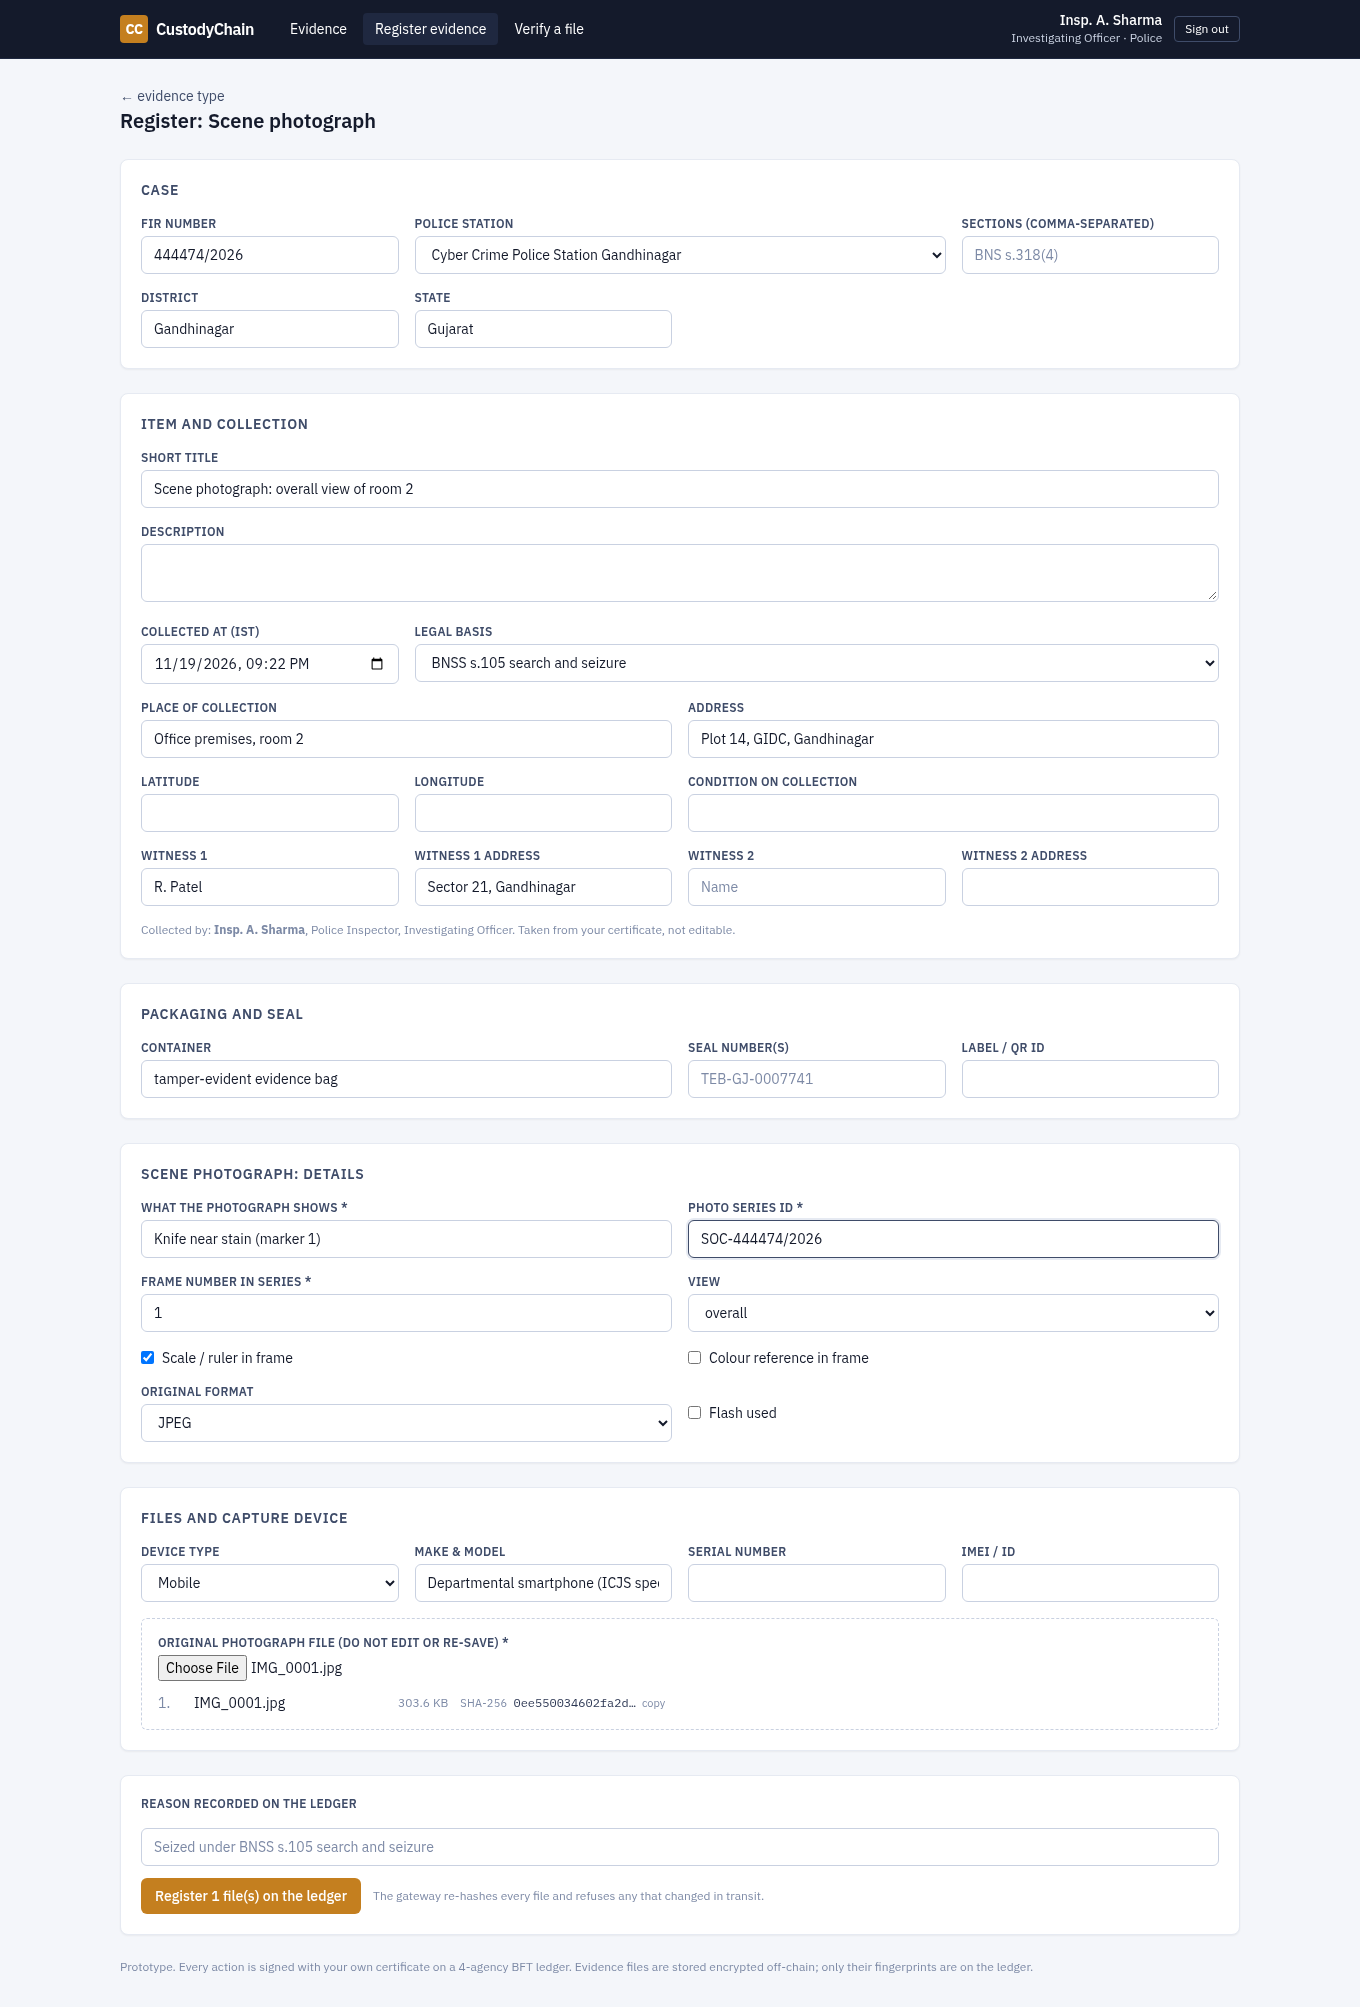
\includegraphics[width=0.49\linewidth,trim=0 520 0 0,clip]{../prototype-screenshots/02-register-photo-hashed-in-browser.png}\hfill
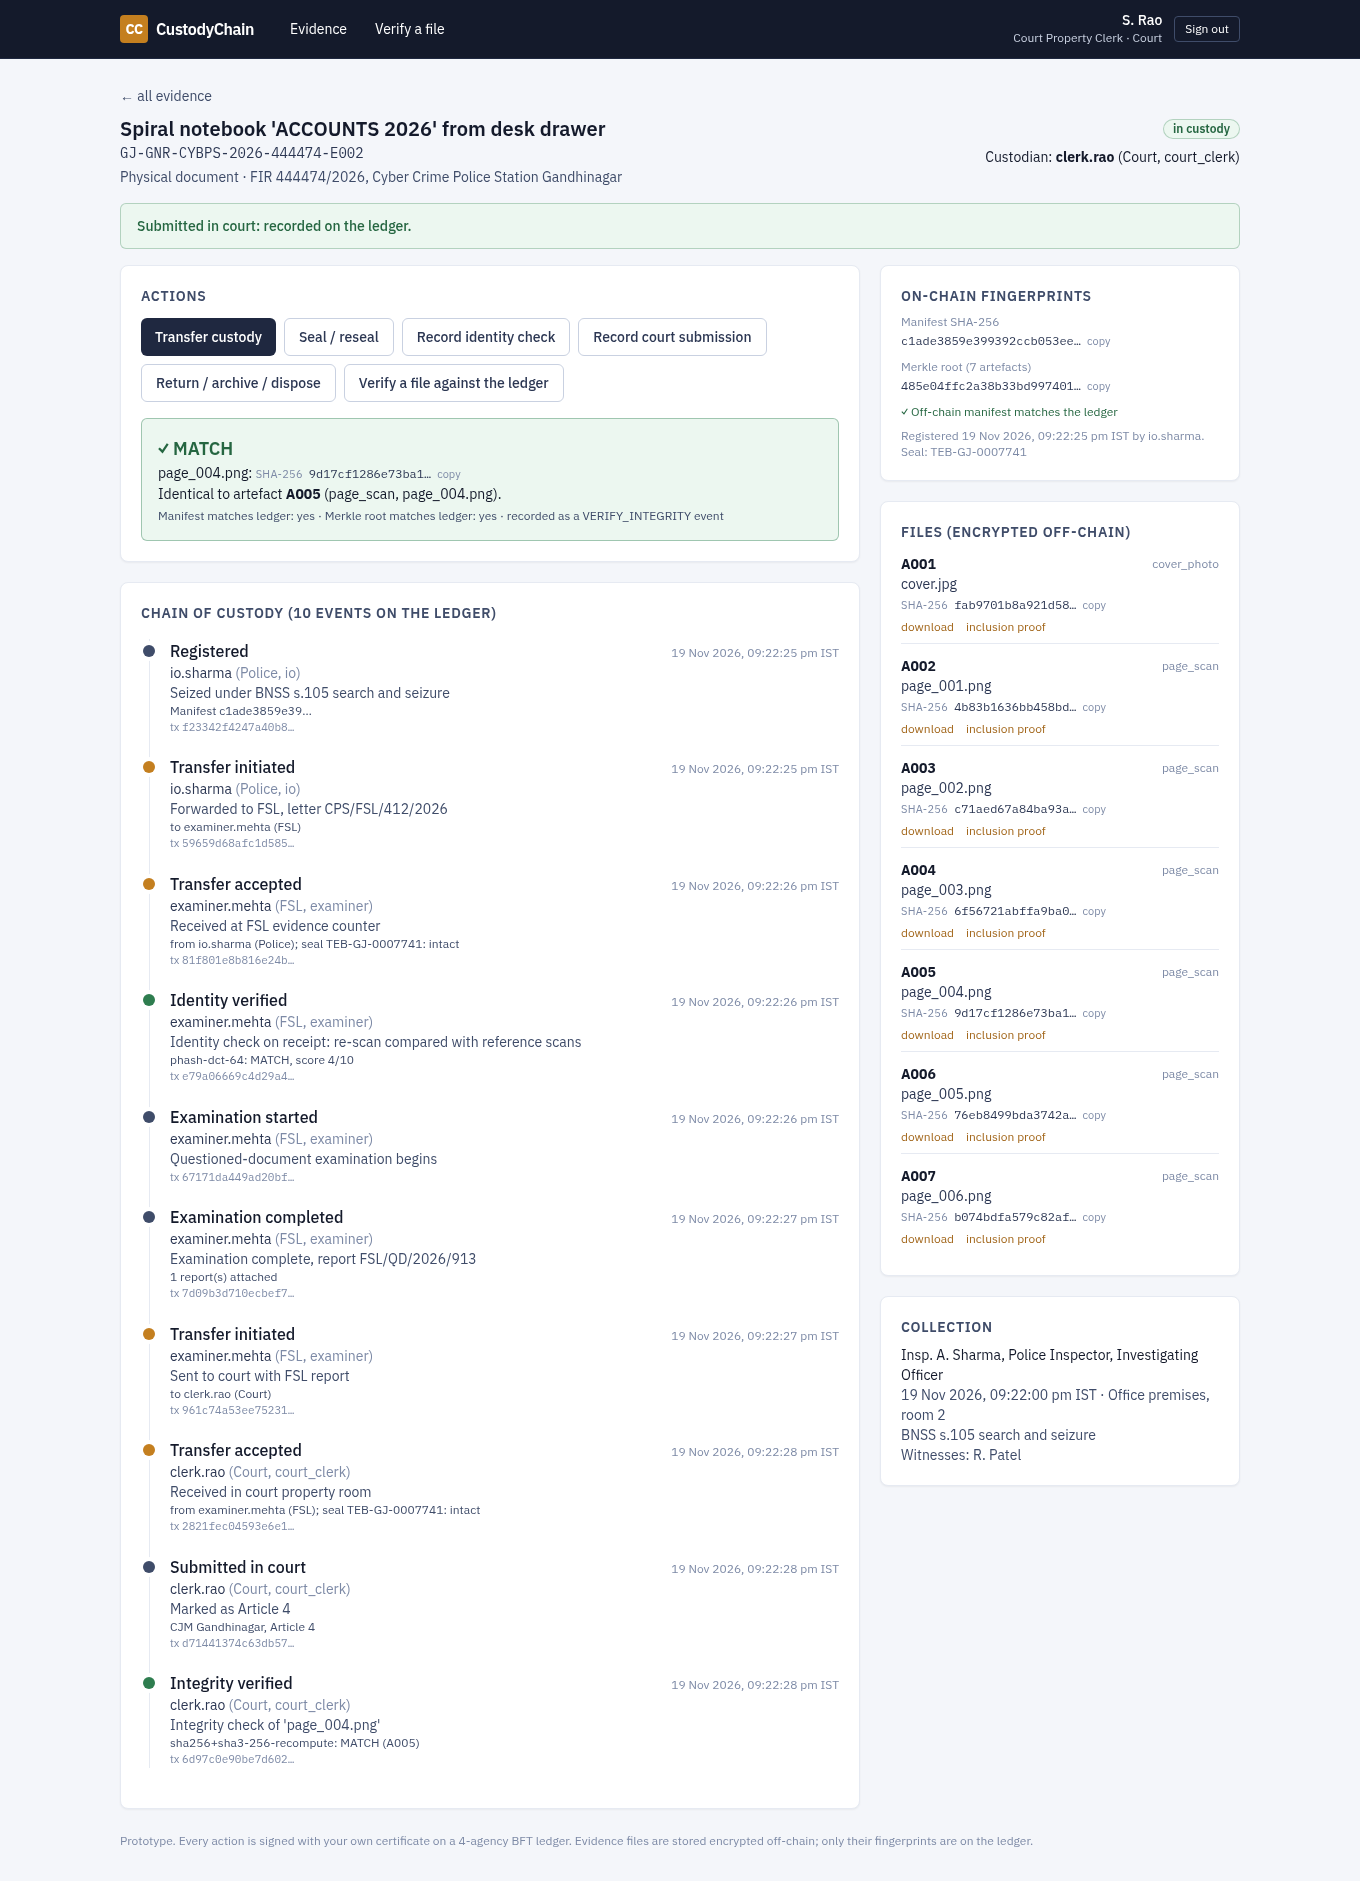
\includegraphics[width=0.49\linewidth,trim=0 900 0 0,clip]{../prototype-screenshots/06-court-evidence-page.png}
\caption{Left: registration form (the file's SHA-256 is shown before upload). Right: an evidence page with the result of a file verification, on-chain fingerprints, encrypted files and the start of the chain of custody.}
\label{fig:ui}
\end{figure}

\subsection{Requirements coverage}
\begin{center}\small
\begin{tabularx}{\linewidth}{@{}lXl@{}}
\toprule
Req. & Implementation & Status \\
\midrule
R1 & SHA-256 in browser and SHA-256 + SHA3-256 in gateway at upload; \code{hashed\_at}/\code{hashed\_on} recorded. Hashing \emph{on the capture device} awaits a capture app (O5). & partial \\
R2 & Schema-validated manifest per item; manifest hash + Merkle root on-chain. & done \\
R3 & Reference fingerprints in the manifest; identity checks recorded with method, scores, thresholds. Thresholds not yet calibrated (O3). & done (uncalibrated) \\
R4 & Actor from certificate, time from transaction, in the contract. & done \\
R5 & Append-only events; corrections as new events. & done \\
R6 & BFT ordering across four agencies; blocks need 3 of 4 consenter signatures; inter-agency transfers need both agencies. & done \\
R7 & Only fingerprints on-chain; salted Merkle leaves; personal data only in encrypted off-chain manifests. & done \\
R8 & Verification page; verification bundle checkable with the independent Python tool. & done \\
R9 & BSA s.63 Part A/B drafts pre-filled from the manifest. & done (draft) \\
R10 & Two digests per artefact; versioned spec and methods. & done \\
\bottomrule
\end{tabularx}
\end{center}
